\documentclass[12pt, a4paper]{article} 
 
\usepackage[utf8]{inputenc}
 

\usepackage[bottom = 8em]{geometry} % to change the page dimensions
\geometry{a4paper} % or letterpaper (US) or a5paper or....
 
\usepackage{graphicx} % support the \includegraphics command and options
 
\usepackage{booktabs} % for much better looking tables
\usepackage{array} % for better arrays (eg matrices) in maths
\usepackage{float}
\usepackage{paralist} % very flexible & customisable lists (eg. enumerate/itemize, etc.)
\usepackage{verbatim} % adds environment for commenting out blocks of text & for better verbatim
\usepackage{subfig} % make it possible to include more than one captioned figure/table in a single float
% These packages are all incorporated in the memoir class to one degree or another...
 
 
 
\usepackage{amsmath, amssymb}% for mathematical symbols
\usepackage[colorlinks=true,linkcolor=black]{hyperref} % for hyperreferences with black color
%\usepackage[T1]{fontenc} % Uncomment for norwegian document
%\usepackage[norsk]{babel} %
 
%%% HEADERS & FOOTERS
\usepackage{fancyhdr} % This should be set AFTER setting up the page geometry
\pagestyle{fancy} % options: empty , plain , fancy
\renewcommand{\headrulewidth}{0pt} % customise the layout...
\lhead{}\chead{}\rhead{}
\lfoot{}\cfoot{\thepage}\rfoot{}

 
%%% SECTION TITLE APPEARANCE
\usepackage{sectsty}
\allsectionsfont{\sffamily\mdseries\upshape} % (See the fntguide.pdf for font help)
% (This matches ConTeXt defaults)
 
%%% ToC (table of contents) APPEARANCE
\usepackage[nottoc,notlof,notlot]{tocbibind} % Put the bibliography in the ToC
\usepackage[titles,subfigure]{tocloft} % Alter the style of the Table of Contents
\renewcommand{\cftsecfont}{\rmfamily\mdseries\upshape}
\renewcommand{\cftsecpagefont}{\rmfamily\mdseries\upshape} % No bold!
 
 
%%% END Article customizations
 
%%% The "real" document content comes below...
 
\title{AI prog 2}
\author{Eivind Hærum \& \ Hong-Dang Lam}
\date{\today} % Activate to display a given date or no date (if empty),
         % otherwise the current date is printed 
 
\begin{document}
\maketitle
%\begin{abstract}
% 
%Abstract
% 
%\end{abstract}
 
\newpage
\tableofcontents
\newpage
 
\section{Working GPS}
Please refer to the delivered code.
We have included a textfile for each problem with some strings of inputs to easily test the program for various configurations.

\section{Diagram}
\begin{figure}[H] 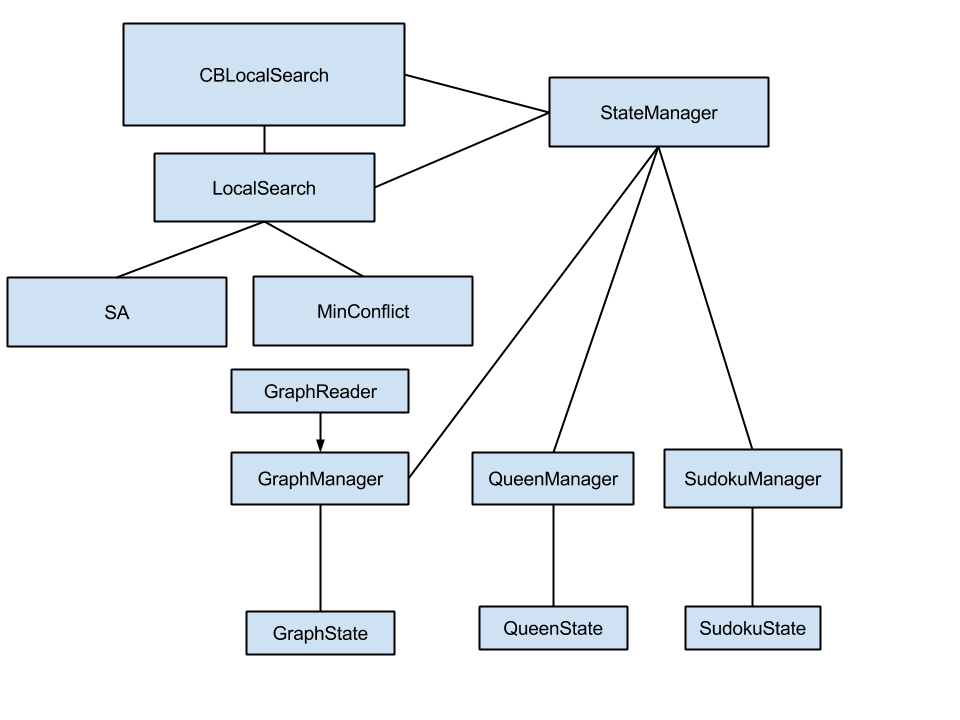
\includegraphics[width=20cm]{2_Diagram}

\caption{Diagram}
\label{diagram}
\end{figure}
\section{Third Puzzle}
Our third puzzle is Sudoku, we have however modified the rules a bit because it makes it easier to implement and we feel that this modification fits the scheme of a scaling constraint satisfaction problem better.\\
The difference between this and the normal Sudoku is the fact that the normal sudoku is usually a board of 3x3 numbered grids (with numbers ranging from and including 1 to and including 9), and the board is pre-filled with some numbers already, these numbers are not allowed to be changed whatsoever.\\
Our modified version starts out with an empty board, follows the same basic rules as the normal Sudoku (meaning there can only be one of each number inside a square, and on each row and column) but we just fill the board in an arbitrary pattern and modify a complete "solution" untill we find one solution that doesn't violate the constraints. We do this by randomly filling each "square" with numbers from 1 to k*k (for instance 1-9 for k=3 - which is the normal sudoku size found in newspapers). We then only swap numbers inside each "square", thus we need only consider conflicts on the rows and columns as the numbers inside each square already meet the contraint that only one of each number may be inside each square. This modified version makes it easy to create scaling problems, as we can simply increase $k$ and make bigger boards, thus making it much more complex and computationally harder.
\\\\
To evaluate the board at a given time, we tally up the number of conflicts for each position with their corresponding column and row, and update a totalCount of all the conflicts.
\\\\
For example if the board looks like this:

\begin{verbatim}

The board

 2  6  4     4  2  8     3  7  1 
 5  9  1     6  3  5     6  9  5 
 7  8  3     7  1  9     2  4  8 

 6  5  1     1  6  4     7  2  4 
 7  9  4     2  8  5     1  3  6 
 2  8  3     7  9  3     9  8  5 

 5  9  2     6  5  1     2  8  7 
 8  6  7     3  2  7     5  4  6 
 4  1  3     8  9  4     9  3  1 

\end{verbatim}

\noindent
Then we have a conflict matrix and a totalCount that looks like this:

\begin{verbatim}

Num of conflicts in total: 100

2 1 2 	1 2 0 	0 0 1 
3 3 1 	2 0 3 	1 1 3 
2 2 2 	2 0 0 	1 1 1 

1 0 2 	1 1 2 	0 0 1 
1 2 1 	0 0 1 	0 1 1 
1 2 3 	1 2 1 	2 2 1 

2 2 1 	1 1 0 	2 1 0 
0 2 1 	0 1 1 	0 1 2 
1 1 3 	0 2 2 	2 2 2 

\end{verbatim}
\noindent
We can for example look at the number 2 in the top leftmost square (pos(0,0)) and see that the conflict matrix states that it has 2 conflicting 2s in total, we can easily verify this by finding the 2 on the same row in the top middle square (pos(0,4)), and the 6 on the same column that is located in the middle leftmost
square (pos(5,0)).
\\
In SA this information is enough to deduce the objective function as we need only count the conflicts on the board and give an appropriate value to such a state. \\
However in Minimum-Conflicts we can use this information more intelligently and look at the conflict matrix to see where we can make a change (I.e. each position where there are 1 or more conflicts), and then pick one of these at random.
\\\\
The way we have opted to choose a neighboring state with use of Minimum-Conflicts is that for the chosen position we temporarily swap with each of the other positions inside the same square, and then tally up the number of conflicts this new position will yield in total (I.e. count both row and column collisions of both the new position with the chosen number and also the old position with the swapped value). This is done by keeping a squareConflict matrix represented such as this:

\begin{verbatim}

Y5X4
[1, 1, 1]
[4, 4, 4]
[1, 2, 4]

\end{verbatim}
\noindent
We see here that the position Y=5, X=4 has been chosen, i.e. the algorithm will traverse the middle square and find the position to swap with that yields the least conflicts.
From the matrix we can see that the set (Y3X3, Y3X4, Y3X5, Y5X3) all yield a total of 1 conflict if swapped to (whereas the original Y5X4 yields 2). The algorithm arbitrarily choose to swap with Y3X5 (so that 9 and 4 switch places) and this is then the resulting board and conflict matrix:

\begin{verbatim}


The board

 2  6  4     4  2  8     3  7  1 
 5  9  1     6  3  5     6  9  5 
 7  8  3     7  1  9     2  4  8 

 6  5  1     1  6  9     7  2  4 
 7  9  4     2  8  5     1  3  6 
 2  8  3     7  4  3     9  8  5 

 5  9  2     6  5  1     2  8  7 
 8  6  7     3  2  7     5  4  6 
 4  1  3     8  9  4     9  3  1 


Num of conflicts in total: 94

2 1 2 	1 2 0 	0 0 1 
3 3 1 	2 0 3 	1 1 3 
2 2 2 	2 0 1 	1 1 1 

1 0 2 	1 1 1 	0 0 0 
1 2 1 	0 0 1 	0 1 1 
1 2 3 	1 0 1 	1 2 1 

2 2 1 	1 1 0 	2 1 0 
0 2 1 	0 1 1 	0 1 2 
1 1 3 	0 1 1 	2 2 2 

\end{verbatim}

\noindent 
The byproduct of this swap is that not only does the swapped values reduce their own conflicts but those previously crashed with as well, thus we manage to reduce the number of total conflicts from 100 down to 94.

\section{Demonstration of K-queen}
%Will be shown on Friday 25. October 2013.
From the assignment text k = 8 is easy, k = 25 is medium and k=1000 is the hard-case, but k = 2500 has a runtime of approximately 1 min by using Minimum-Conflicts.
\\\\
Internally the board is represented as a one dimensional matrix where each index represents the column position for the given row. For example the board matrix:

\begin{verbatim}

[5,3,0,4,7,1,6,3]

\end{verbatim}
\noindent
means that on f.ex row 0 the queen is placed on column 5. The more readable representation (the printed board) would then look like this:

\begin{verbatim}

[0, 0, 0, 0, 0, 1, 0, 0]
[0, 0, 0, 1, 0, 0, 0, 0]
[1, 0, 0, 0, 0, 0, 0, 0]
[0, 0, 0, 0, 1, 0, 0, 0]
[0, 0, 0, 0, 0, 0, 0, 1]
[0, 1, 0, 0, 0, 0, 0, 0]
[0, 0, 0, 0, 0, 0, 1, 0]
[0, 0, 0, 1, 0, 0, 0, 0]

\end{verbatim}

\noindent
Because we have opted to use a one dimensional matrix internally, the creation and alteration of a state is both easier and faster than if we had to keep track a bunch of 1s and 0s in a two dimensional matrix. Now we simply need to change the number for a given index and traverse the matrix to count up conflicts. The conflict matrix is thus also a one dimensional matrix where each index tells us how many crashes the queen at a given row has. For our given board it would look like this:

\begin{verbatim}

[0,1,0,0,0,1,0,2]

\end{verbatim}

\noindent
For SA create children where we chose one random row and move the queen on that row to a random column. The idea here is to alter the states slightly in the hope of getting closer to a goal state. The way SA determines the value of a particullar state is by counting the crashes in total and giving a value based on this. 
\\
However if we run Minimum-Conflict, and on this iteration randomly choose to alter the position for the queen at row 7 we would have to check each position for the queen on that given row. For this purpose we have yet another one dimensional matrix which counts up how many conflicts the move would produce if we opted to move to a particullar column. For this row we would have the NumberOfColumnConflict matrix appearing like this:

\begin{verbatim}

[2,1,0,2,2,3,1,2]

\end{verbatim}
\noindent
Thus the algorithm would move the queen at row 7 from column 3 to 2 and thereby reaching a goal state. 


\section{Result table of K-queens, and a description of an easy-case}
One of the solutions found for the easy-case (k=8)

\begin{verbatim}
QueenManager k=8
The board 
[0, 0, 0, 0, 0, 1, 0, 0]
[0, 0, 0, 1, 0, 0, 0, 0]
[1, 0, 0, 0, 0, 0, 0, 0]
[0, 0, 0, 0, 1, 0, 0, 0]
[0, 0, 0, 0, 0, 0, 0, 1]
[0, 1, 0, 0, 0, 0, 0, 0]
[0, 0, 0, 0, 0, 0, 1, 0]
[0, 0, 1, 0, 0, 0, 0, 0]

\end{verbatim}
\noindent
Final statistic for 20 runs with a maximum of 10000 iterations with min-conflict (there is no need to include average and standard deviation for evaluation as it solves everything each run. Though it does happend on a few occations that the easy problems gets stuck):\\
\begin{center}
  \begin{tabular}{| l | c c c|}
    \hline
    Hardness: &\textbf{Easy} & \textbf{Medium} & \textbf{Hard} \\ \hline
    Average iterations reaching goal: & 72.9& 64.7 & 695.55\\
    Average iterations per run:  & 72.9 & 64.7 & 695.55\\
    Standard deviation for iterations $\sigma$ & 73 & 38 & 21.5\\
    Fewest iteration: & 9 & 20& 659\\ 
    Most iterations: & 276 & 185& 747\\ 
    Number of goal reached: & 20/20 & 20/20 & 20/20\\
    Total iterations: & 1458 & 1294& 13911\\
    Total iterations where goal is reached: & 1294 & 2099& 13911\\
    Total time spent: & 87ms & 120ms & 128924ms\\
    \hline
  \end{tabular}
\end{center}
\noindent
Final statistic for 20 runs with a maximum of 10000 iterations with SA:\\
\begin{center}
  \begin{tabular}{| l | c c c|}
    \hline
    Hardness: &\textbf{Easy} & \textbf{Medium} & \textbf{Hard} \\ \hline
    Average iterations reaching goal: & 547.35& N/A & N/A\\
    Average iterations per run:  & 447.35 & 10000 & 10000\\
    Average F value: & 1.0 & 0.772 & 0.50\\
    Standard deviation of F: & 0.0 & 0.05 & 0.012\\
    Standard deviation for iterations $\sigma$ & 567.41 & 0 & 0\\
    Fewest iterations: & 9 & N/A & N/A\\ 
    Most iterations: & 2323 & N/A& N/A\\ 
    Number of goal states reached: & 20/20 & 0/20 & 0/2\\
    Total iterations: & 10947 & 200000 & 20000\\
    Total iterations where goal is reached: & 10947 & N/A& N/A\\
    Total time spent: & 301ms & 14957ms & 1644710ms\\
    \hline
  \end{tabular}
\end{center}
The Hard problem for k-queens using the SA algorithm takes around 13-14 minutes, so we couldn't really do 20 runs of this one because it takes way too much time, that's why we decided to only run 2 runs of the hard problem to have some data to document. Due to the enormous search space SA struggles to find a good way to make a describing objective value when there is so many conflicts. Thus it has a problem with climbing closer to a solution. 

\section{Demonstration of Graph-color}
%Will be shown on Friday 25. October 2013.
We have decided that number 1 is easy, 2 is medium and 3 is hard-case.  These numbers correspond to the txt file given inside the project - that is 1 corresponds to \textit{graph-color-1.txt} etc. (do note that we swapped the numbers 1 and 2 of the provided files).\\
The first "easy" one have a 40 nodes/countries and 67 edges/countries bordering each other, the second medium one have 40 nodes and 97 edges whilst the hardest problem have 500 nodes with 1009 edges.\\ 
We decided to classify these problems as such because it is more logical that the more edges and nodes you have, the harder the problem becomes. It's also the only input we have for this problem.
This problem is also known as vertex-coloring, which is a problem where you have to color every node with a color so that none of its neighbor have the same color.\\
The data we got is explained here:\\ \href{http://www.idi.ntnu.no/emner/it3105/materials/data/graph-color-format.txt}{http://www.idi.ntnu.no/emner/it3105/materials/data/graph-color-format.txt},
as you can see, these nodes are provided with coordinates. These coordinates are mostly there for the visual representation if needed, it's not needed for the actual problem, this is because there's no need for information \textbf{where} the nodes are located as long as we know how the edges are connected. For this task, we've decided to use a neighbor-matrix to represent the nodes and the edges, this is represented by a 2-dimensional boolean array where a \textit{True} indicates an edge between a node \textit{i} and node \textit{j} ($i \neq j$) and an int array which contains the colors of each node. For instance, if we have 3 nodes which are all connected, we would have:\\
Matrix:\\
\begin{center}
\begin{verbatim}
[0,1,1]
[1,0,1]
[1,1,0]
\end{verbatim}
\end{center}
The nodes array which contains the colors could be:
\begin{center}
\begin{verbatim}
[1,0,0]
\end{verbatim}
\end{center} (nodes where the first node is color 1 and the rest is color 0)\\
This would give us a conflict array which looked like this:\\
\begin{center}
\begin{verbatim}
[0,1,1]
\end{verbatim}
\end{center}
Which means that all node 2 and 3 have each 1 conflict each with eachother, because both of them have a neighbour with the same color as itself. We calculate the temperature (F) by calculating the number of crashes in total and using this formula: $F = 1- \frac{crashes}{number of Nodes}$ \\
For the minconflict algorithm we take one randomly chosen node given that the chosen node was either not chosen last iteration or a color change was applied to this node the last iteration. This randomly chosen node then calculates how many conflicts it will have for the four colors and stores this in an array of this node's conflicts. We then try to find the lowest conflict for this node, and this happens to be the same color as the one it started with then we either change to a randomly chosen color that doesn't increase the number of conflicts or tell the next iteration to ignore this node if it happens to be the original color that yields the lowest conflict for this node. This will ensure enough "jiggling" to make sure the coloring doesn't get tangled. 

\section{Result table of Graph-Coloring, and the description of an easy-case}
One of the runs and its solution printed out, the N indicates which node we are looking at and the C tells us which color this node is. We have used numbers to represent the colors because this is easier to work with.\\
\begin{verbatim}
GraphManager: graph-color-1.txt

num of conflicts in total: 0
N = Node C = Color
N:0 C:2| N:1 C:1 
N:1 C:1| N:0 C:2 N:2 C:0 N:3 C:3 N:4 C:2 
N:2 C:0| N:1 C:1 N:3 C:3 N:4 C:2 
N:3 C:3| N:1 C:1 N:2 C:0 N:4 C:2 
N:4 C:2| N:1 C:1 N:2 C:0 N:3 C:3 N:5 C:3 
N:5 C:3| N:4 C:2 N:6 C:0 
N:6 C:0| N:5 C:3 N:7 C:2 N:8 C:3 
N:7 C:2| N:6 C:0 N:8 C:3 N:9 C:1 N:10 C:0 
N:8 C:3| N:6 C:0 N:7 C:2 N:9 C:1 N:10 C:0 
N:9 C:1| N:7 C:2 N:8 C:3 N:10 C:0 N:11 C:2 
N:10 C:0| N:7 C:2 N:8 C:3 N:9 C:1 N:11 C:2 N:12 C:3 
N:11 C:2| N:9 C:1 N:10 C:0 N:12 C:3 
N:12 C:3| N:10 C:0 N:11 C:2 N:13 C:2 
N:13 C:2| N:12 C:3 N:14 C:3 
N:14 C:3| N:13 C:2 N:15 C:0 N:16 C:1 
N:15 C:0| N:14 C:3 N:16 C:1 N:18 C:3 
N:16 C:1| N:14 C:3 N:15 C:0 N:17 C:2 N:18 C:3 N:19 C:0 
N:17 C:2| N:16 C:1 N:18 C:3 N:19 C:0 
N:18 C:3| N:15 C:0 N:16 C:1 N:17 C:2 N:19 C:0 N:20 C:2 
N:19 C:0| N:16 C:1 N:17 C:2 N:18 C:3 N:20 C:2 N:22 C:1 
N:20 C:2| N:18 C:3 N:19 C:0 N:21 C:0 N:22 C:1 
N:21 C:0| N:20 C:2 N:22 C:1 
N:22 C:1| N:19 C:0 N:20 C:2 N:21 C:0 N:23 C:2 
N:23 C:2| N:22 C:1 N:24 C:3 N:26 C:0 
N:24 C:3| N:23 C:2 N:25 C:1 N:26 C:0 
N:25 C:1| N:24 C:3 N:26 C:0 N:27 C:3 
N:26 C:0| N:23 C:2 N:24 C:3 N:25 C:1 N:27 C:3 
N:27 C:3| N:25 C:1 N:26 C:0 N:28 C:0 N:29 C:1 N:30 C:2 
N:28 C:0| N:27 C:3 N:29 C:1 N:30 C:2 N:31 C:3 
N:29 C:1| N:27 C:3 N:28 C:0 N:30 C:2 N:31 C:3 
N:30 C:2| N:27 C:3 N:28 C:0 N:29 C:1 N:31 C:3 
N:31 C:3| N:28 C:0 N:29 C:1 N:30 C:2 N:32 C:2 
N:32 C:2| N:31 C:3 N:33 C:0 N:34 C:1 
N:33 C:0| N:32 C:2 N:34 C:1 N:35 C:2 
N:34 C:1| N:32 C:2 N:33 C:0 N:35 C:2 
N:35 C:2| N:33 C:0 N:34 C:1 N:36 C:1 
N:36 C:1| N:35 C:2 N:37 C:3 
N:37 C:3| N:36 C:1 N:38 C:2 N:39 C:1 
N:38 C:2| N:37 C:3 N:39 C:1 
N:39 C:1| N:37 C:3 N:38 C:2 

\end{verbatim}
\noindent
Final statistic for 20 runs with a maximum of 10000 iterations with min-conflict (there is no need to include average and standard deviation for evaluation as it solves everything each run):\\
\begin{center}
  \begin{tabular}{| l | c c c|}
    \hline
    Hardness: &\textbf{Easy} & \textbf{Medium} & \textbf{Hard} \\ \hline
    Average iterations reaching goal: & 21.45& 104.95& 646.4\\
    Average iterations per run:  & 21.45 & 104.95 &  646.4\\
    Standard deviation for iterations $\sigma$ & 10.14 & 42.96 & 67.16\\
    Fewest iterations: & 11 & 45& 493\\ 
    Most iterations: & 59 & 191& 766\\ 
    Number of goal states reached: & 20/20 & 20/20 & 20/20\\
    Total iterations: & 429 & 2099& 12928\\
    Total iterations for goal states: & 429 & 2099& 12928\\
    Total time spent: & 97ms& 149ms & 9336ms\\
    \hline
  \end{tabular}
\end{center}
Final statistic for 20 runs with a maximum of 10000 iterations with SA: \\
\begin{center}
  \begin{tabular}{| l | c c c|}
    \hline
    Hardness: &\textbf{Easy} & \textbf{Medium} & \textbf{Hard} \\ \hline
    Average iterations reaching goal: & 9004.55& 9417.5 & N/A\\
    Average iterations per run:  & 9004.55 & 9941.75 &  10000\\
    Average F value: & 1.0 & 0.74 & 0.69\\
    Standard deviation of F: & 0.0 & 0.13& 0.02\\
    Standard deviation for iterations $\sigma$ & 386.74 & 213.98 & 0\\
    Fewest iteration: & 8158 & 9027& N/A\\ 
    Most iterations: & 9924 & 9808& N/A\\ 
    Number of goal states reached: & 20/20 & 2/20 & 0/20\\
    Total iterations: & 180091 & 198835& 200000\\
    Total iterations for goal states: & 18835 & 2099& N/A\\
    Total time spent: & 22976ms & 28580ms & 2873082ms\\
    \hline
  \end{tabular}
\end{center}


\section{Demonstration of the modified Sudoku}
%Will be shown on Friday 25. October 2013.
We have decided that k = 2 is easy case, 3 is medium, 9 is hard. 
We have decided to use these \textit{k}s because of the runtime, the k for the hard problem runs in 1 minutes - which is what the assignment text wants the runtime of a hard problem to be. The k = 9 problem runs in around 30 second per run, but the next k = 10 runs in ca. 90 seconds for the min conflict algorithm. That's why we decided to use k = 9 because it takes WAY too long per run for the SA algorithm, and we want to be able to deliver in time.
\\\\
For a detailed description of how this problem was solved internally see section 3

\section{Result table of modified Sudoku, and description of an easy-case}
\begin{verbatim}
The board

 4  2     1  3 
 1  3     2  4 

 3  1     4  2 
 2  4     3  1 
 
Iterations for this run:9
Time spent on this run: 1ms
\end{verbatim}

\noindent
Final statistic for 20 runs with a maximum of 10000/10000/30000 iterations (easy,medium,hard respectivly. Hard requires more iterations due to the size of the search space, but its still quite fast) with Minimum Conflicts (Solves everything so no need for evalution fields):

\begin{center}
  \begin{tabular}{| l | c c c|}
    \hline
    Hardness: &\textbf{Easy} & \textbf{Medium} & \textbf{Hard} \\ \hline
    Average iterations reaching goal: & 8.45& 79.65 & 18285\\
    Average iterations per run:  & 8.45 & 79.65 & 18285\\
    Standard deviation for iterations $\sigma$ & 4.92 & 26.52 & 1205.73\\
    Fewest iterations: & 2 & 35& 16503\\ 
    Most iterations: & 19 & 147& 21297\\ 
    Number of goal states reached: & 20/20 & 20/20 & 20/20\\
    Total iterations: & 169 & 1593& 365700\\
    Total iterations goal states: & 169 & 1593& 365700\\
    Total time spent: & 19ms & 113ms & 503847ms\\
    \hline
  \end{tabular}
\end{center}
\noindent
SA: (we've taken 20000 as the maximum iteration for the medium one, because it's still fast enough and there might be a chance of solving it)\\
%HARD ONE IS NOT COMPLETED, STILL RUNNING ON MY PC
\begin{center}
  \begin{tabular}{| l | c c c|}
    \hline
    Hardness: &\textbf{Easy} & \textbf{Medium} & \textbf{Hard} \\ \hline
    Average iterations reaching goal: & 15.8& N/A & N/A\\
    Average iterations per run:  & 15.8 & 20000 & 10000\\
    Average F value: & 1.0 & 0.86 & 0.800\\
    Standard deviation of F: & 0.0 & 0.028 & 0.0013\\
    Standard deviation for iterations $\sigma$ & 15.47 & 0 & 0\\
    Fewest iterations: & 1 & N/A & N/A\\ 
    Most iterations: & 48 & N/A& N/A\\ 
    Number of goal reached: & 20/20 & 0/20 & 0/10\\
    Total iterations: & 316 & 400000& 100000\\
    Total iterations for goal states: & 316 & N/A& N/A\\
    Total time spent: & 71ms & 54755ms & 3038673ms\\
    \hline
  \end{tabular}
\end{center}
\noindent
\\
We opted to only run the SA algorithm 10 times on the hard problem due to the very long runtime. It struggles to find a solution even on the medium problem. This algorithm just is not cut out to find a solution in such a big and diverse search space. It may find a somewhat decent solution but it has a very hard time reaching a goal. 

\end{document}